% arara: latexmk: { options: [ '-pdf' ] }
% arara: latexmk: { options: ['-c' ] }
\documentclass{article}
\title{AP Physics C Test 2}
\author{Henry Beveridge}

\date{March 18, 2025}
\usepackage{tikz}
\usepackage{amsmath}


\begin{document}

\maketitle

\section{}

\large\textbf{a)} Diagram of the system:

\begin{center}
    \begin{tikzpicture}
        \draw[dashed,<->] (0,-4) -- (0,4);
        \draw[dashed,<->] (-4,0) -- (4,0);
    
        \fill (0,3) circle (4pt);
        \node[anchor=west] at (0.2,3) {$M$};
        \node[anchor=east] at (-0.2,3) {$+y$};
        \fill (0,-3) circle (4pt);
        \node[anchor=west] at (0.2,-3) {$M$};
        \node[anchor=east] at (-0.2,-3) {$-y$};

        \fill (1,0) circle (2pt);
        \node[anchor=south west] at (1,0.2) {$m$};
        \node[anchor=north] at (1,-0.2) {$x_0$};
    \end{tikzpicture}
\end{center}

Diagram of forces on $m$:

\begin{center}
    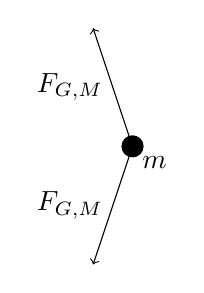
\begin{tikzpicture}
        \fill (0,0) circle (4pt) node[anchor=north west] {$m$};
        \draw[->] (0,0) -- (-0.5,-1.5) node[midway, anchor=east] {$F_{G,M}$};
        \draw[->] (0,0) -- (-0.5,1.5) node[midway, anchor=east] {$F_{G,M}$};
    \end{tikzpicture}
\end{center}

\vspace{1cm}
\large\textbf{b)} The $y$ components of the net force cancel out because for both masses the mass is the same and the distance is the same. Thus, we only have to consider the $x$ component. More so, the $x$ components of each gravitational force are equal, so we can just compute one.

\begin{align*}
    F_{g,M} &= G\frac{Mm}{r^2} = G\frac{Mm}{x^2+y^2}\\
    F_{g,M,x} &= G\cdot\text{cos}(\theta)\frac{Mm}{x^2+y^2} \\
    &= G\frac{Mm}{x^2+y^2}\cdot\frac{x}{\sqrt{x^2+y^2}}\\
    F_{g,M,x}&= G\frac{Mm x}{(x^2+y^2)^{3/2}}
\end{align*}

Thus,
$$
||F_{net}|| = 2G\frac{Mm x}{(x^2+y^2)^{3/2}}
$$

\vspace{1cm}
\large\textbf{c)} Since there is only motion in the $x$ direction, we can just use Newton's second law in the $x$ direction.

\begin{align*}
    F_{net} &= ma \\
    -2G\frac{Mm x}{(x^2+y^2)^{3/2}} &= ma \\
    -\frac{2G\frac{Mm x}{(x^2+y^2)^{3/2}}}{m} &= a\\
    -\frac{2GM}{(x^2+y^2)^{3/2}}x &= \frac{d^2x}{dt^2}
\end{align*}

\vspace{1cm}
\large\textbf{d)} Using the approximation of $\sqrt{x^2+y^2}=y$ because $x<<y$:

\begin{align*}
    \frac{d^2 x}{dt^2} &= -\frac{2GM}{({x^2+y^2})^{3/2}}x \\
    &\approx -\frac{2GM}{y^3}x \\
    x(t) &= A\cos(\omega t + \phi) \\ 
    &\text{where } \omega = \sqrt{\frac{2GM}{y^3}}\\
    &\text{and } \phi = 0 \\
    &\text{and } A = x_0 \text{ both because it starts at } x_0.\\
    x(t) &= x_0\cos\left(\sqrt{\frac{2GM}{y^3}}t\right)
\end{align*}

\vspace{1cm}
\large\textbf{e)} The next moment when it is at rest is when it reaches $-x_0$, so we solve the above equation. JK, this time is just half the period.

\begin{align*}
    t_{rest} &= \frac{1}{2}\cdot\frac{2\pi}{\omega} \\
    &= \frac{\pi}{\omega} \\
    t_{rest} &= \pi\sqrt{\frac{y^3}{2GM}} \\
\end{align*}

\newpage
\section{}

\vspace{1cm}
\large\textbf{a)} Yay simple mechanics

\begin{align*}
    v_f^2 &= v_i^2 + 2a\Delta x \\
    v_f^2 &= 2(10)(.2) \\
    v_f &= 2\,\frac{\text{m}}{\text{s}}
\end{align*}

\vspace{1cm}
\large\textbf{b)} Equilibrium is when the net force is 0 on the block, so to find the new equilibrium position we find when force of gravity equals the spring force.
\begin{align*}
    F_{g} &= F_{spring} \\
    mg &= kx \\
    x &= \frac{mg}{k} \\
    &= \frac{(0.05)(10)}{5} \\ 
    x &= 0.1 \, \text{m}
\end{align*}

So, the new equilibrium position is 0.1 m below the block.

\vspace{1cm}
\large\textbf{c)} For this, we need to calculate when the kinetic energy of the block plus the gravitational potential energy equals the potential energy of the spring.

\begin{align*}
    KE + PE_g &= PE_{spring}\\
    \frac{1}{2}mv^2 + mgx &= \frac{1}{2}kx^2 \\
    \frac{1}{2}(0.05)(2^2) + (0.05)(10)(x) &= \frac{1}{2}(5)(x^2) \\
    0.1 + 0.5x &= 2.5x^2 \\
    2.5x^2 - 0.5x - 0.1 &= 0 \\
\end{align*}

Solve for $x$ using the quadratic formula:

\begin{align*}
    x &= \frac{-b \pm \sqrt{b^2 - 4ac}}{2a} \\
    &= \frac{-(-0.5) \pm \sqrt{(-0.5)^2 - 4(2.5)(-0.1)}}{2(2.5)} \\
    &= \frac{0.5 \pm \sqrt{0.25 + 1}}{5} \\
    &= \frac{0.5 \pm \sqrt{1.25}}{5} \\
    &\approx \frac{0.5 \pm 1.118}{5} \\
    &\approx 0.324 \\
\end{align*}

Thus, about 0.324 m below the block's position at landing.

\vspace{1cm}

\large\textbf{d)} For period, we can use the equation for the period of a mass on a spring in SHM:

\begin{align*}
    T_1 &= 2\pi\sqrt{\frac{m}{k}} \\
    T_2 &= 2\pi\sqrt{\frac{2m}{k}} \\
    T_2 &= \sqrt{2}T_1
\end{align*}

For amplitude, it's a little more involved. Since the system is essentially in SHM, the maximum speed would be found at the new equilibrium position. In SHM, speed at this point is just $A\omega$.

First, I'll find the new equilibrium position in terms of the old one:

\begin{align*}
    2mg &= kx \\
    \frac{2mg}{k} &= x \\
    x_{eq,2} &= 2x_{eq,1} \\
\end{align*}

Then, I'll find the speed on impact with the spring in terms of the first situation:

\begin{align*}
    m_1v_1+m_2v_2 &= (m_1+m_2)v_f \\
    (0.05)(2) + (0.05)(0) &= (0.1)(v_f) \\
    0.1 &= 0.1v_f \\
    v_f &= 1 \frac{\text{m}}{\text{s}} \\
    v_{f,2} &= \frac{1}{2}v_{f,1} 
\end{align*}

So, we can find the ratios of $v_{max}$ and ${\omega}$. First $v_{max}$ is the same as $v_{eq}$ because there's the most kinetic energy there:

\begin{align*}
    KE_{eq} &= PE_{spring} + KE_{initial} \\
    \frac{1}{2}mv_{eq}^2 &= \frac{1}{2}kx_{eq}^2 + \frac{1}{2}mv_1^2 \\
    v_{eq}^2 &= \frac{m}{k} g^2 + v_1^2 \\
    v_{eq,2}^2 &= 2 \frac{m}{k} g^2 + \frac{1}{4}v_1^2 \\
    \left(\frac{v_{eq,2}}{v_{eq}}\right)^2 &= \frac{2\frac{m}{k}g^2 + \frac{1}{4}v_1^2}{\frac{m}{k}g^2 + v_1^2} \\
    &= \frac{2\frac{0.05}{5}10^2 + \frac{1}{4}(2)^2}{\frac{0.05}{5}10^2 + (2)^2} \\
    &= \frac{3}{5} \\
    \frac{v_{eq,2}}{v_{eq}} &= \sqrt{\frac{3}{5}}
\end{align*}

Next $\omega$:

\begin{align*}
    \left(\frac{\omega_2}{\omega_1}\right)^2 &= \frac{\frac{k}{2m}}{\frac{k}{m}} \\
    &= \frac{1}{2} \\
    \frac{\omega_2}{\omega_1} &= \frac{1}{\sqrt{2}}
\end{align*}

So, we can find the ratio of amplitude:

\begin{align*}
    \frac{A_2}{A_1} &= \frac{v_{eq,2}}{\omega_2}\cdot\frac{\omega_1}{v_{eq}} \\
    &= \sqrt{\frac{3}{5}}\cdot\sqrt{2} \\
    &= \sqrt{\frac{6}{5}} \\
\end{align*}

So, $A_2 = A_1\sqrt{\frac{6}{5}}$.

\newpage
\section{}

We can use the equation for the period of a physical pendulum, we know that the only thing that can change is the moment inertia and the distance to center of mass. Mass stays the same, and all distances decrease, including those in moment of inertia.

\begin{align*}
    T_2 &= 2\pi\sqrt{\frac{I_2}{mgl_2}} \\
    &= 2\pi\sqrt{\frac{I/4}{mgl/2}} \\
    T_2 &= \frac{T_1}{\sqrt{2}}
\end{align*}

\newpage
\section{}

\textbf{a)} We can use the equation for orbital speed to solve for the radius of the largest asteroid we can throw things into orbit on.

But first, we need to find the mass of the asteroid in terms of $r$:
\begin{align*}
    \rho &= \frac{M}{V} \\
    &= \frac{M}{\frac{4}{3}\pi r^3} \\
    M &= \rho\cdot\frac{4}{3}\pi r^3 \\
\end{align*}

Then we can solve!

\begin{align*}
    v &= \sqrt{\frac{GM}{r}} \\
    v_t &= \sqrt{\frac{G\rho\cdot\frac{4}{3}\pi r^3}{r}} \\
    v_t &= r \sqrt{\frac{4\pi G\rho}{3}} \\
    r &= \frac{v_t}{\sqrt{\frac{4\pi G\rho}{3}}} \\
    r &= \frac{v_t\sqrt{3}}{\sqrt{4\pi G\rho}} \\
\end{align*}

\vspace{1cm}
\textbf{b)} We can use energy to solve for this

\begin{align*}
    \frac{1}{2}mv_e^2 &= \frac{GMm}{R} \\
    v_e^2 &= \frac{2GM}{R} \\
\end{align*}

Kinetic energy is 16 times less with the new speed, so the max height is 16 times less as well.

$$
h_{max} = \frac{R}{16}
$$

\end{document}
